\subsubsection{Threshold Value Determination}
\label{subsubsec:threshold}
% \todo[inline]{Citations}

Ideally, the mean absolute difference between two consecutive unchanged frames is zero.
This is not the case, however, due to image noise and other environmental influences such as \SI{50}{Hz} flickering of the ambient light intensity.
A suitable threshold value must therefore be determined.
% For this purpose, the first eight mean absolute differences $\overline{\text{MD}}$ are averaged to determine the threshold value.
% For this purpose, the first eight mean absolute differences $\overline{\text{MD}}$ are averaged and multiplied by a multiplier to determine the threshold value.
For this purpose, the first eight mean absolute differences $\overline{\text{MD}}$ are used to determine the threshold value.
They are averaged and multiplied by a multiplier, as show in figure \ref{fig:threshold}.
At a frame rate of \SI{200}{fps} this results in a short start-up delay of \SI{40}{ms}.

\begin{figure}[h]
  \centering
  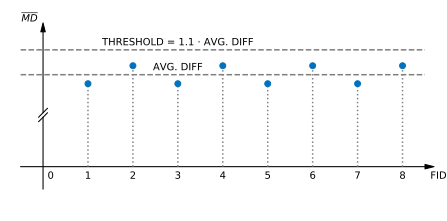
\includegraphics[width=0.75\textwidth]{threshold}
  \caption{Determination of the threshold value from eigth mean absolute differences}
  \label{fig:threshold}
\end{figure}
